Conceptually, query evaluation in PIP is broken up into two components: Query and Sampling.  PIP relies on Postgres to evaluate queries; As described in Section \ref{sec:background}, a query rewriting pass suffices to translate c-tables relational algebra extensions into traditional relational algebra.  Details on how query rewriting is implemented are provided in Section \ref{sec:implementation}.  

As the query is being evaluated, special sampling operators in the query are used to transform random variable expressions into histograms, expectations, and other moments.  Both the computation of moments and probabilities in the general case reduces to numerical integration, and a dominant technique for doing this is Monte Carlo simulation. The approximate computation of expectation
\begin{equation}
E[\chi_\phi \cdot (h \circ t)] =
\frac{1}{n} \cdot \sum_{i=1}^n p(\vec{y}_i) \cdot \chi_\phi(\vec{y}_i) \cdot
h(t(\vec{y}_i))
\end{equation}
faces a number of difficulties.  In particular, samples for which $\chi_{\phi}$ is zero do not contribute to an expectation.  If $\phi$ is a very selective condition, most samples do not contribute to the summation computation of the approximate expectation.  (This is closely related to the most prominent problem in online aggregation systems \cite{OnlineAggregation,DBO}, and also in MCDB).

\begin{example}\em 
Consider a row containing the variable 
$$[Y \Rightarrow Normal(\mu=5,\sigma^2=10)]$$
and the condition predicate $(Y > -3)$ and $(Y < 2)$.  The expectation of the variable $Y$ in the context of this row is not $5$.  Rather the expectation is taken only over samples of $Y$ that fall in the range $(-3,2)$, (coming out to approximately $0.17$).  
\end{example}

\subsection{Sampling Techniques}
\label{subsec:samplingTechs}

\paragraph{Rejection Sampling}
One straightforward approach to this problem is to perform rejection sampling; sample sets are repeatedly generated until a sufficient number of viable (satisfying) samples have been obtained.  %Note that this is not strict rejection sampling, samples for with $\chi_{\phi}$ is zero count towards the number or samples $n$ by which we average.  

However, without scaling the number of samples taken based on $E[\chi_\phi]$, information can get very sparse and the approximate expectations will have a high relative error.  Unfortunately, as the probability of satisfying the constraint drops, the work required to produce a viable sample increases.   Consequently, any mechanism that can improve the chances of satisfying the constraint is beneficial.

\paragraph{Sampling using inverse CDFs}
\label{subsec:icdf}
As an alternative to generator functions, PIP can also use the inverse-transform method \cite{lawSimulation}.  If available, the distribution's inverse-CDF function is used to translate a uniform-random number in the range $[0,1]$ to the variable's distribution.  

This technique makes constrained sampling more efficient.  If the uniform-random input is selected from the range $[CDF(a), CDF(b)]$, the generated value is guaranteed to fall in the range $[a, b]$.  Even if precise constraints can not be obtained, this technique still reduces the volume of the sampling space, increasing the probability of getting a useful sample.

%In the event that the inverse CDF is available, but the CDF is not, this technique may still be used.  Instead of sampling from the range $(CDF(lower), CDF(upper))$, we sample $x \in (L,H)$ where $L$ is initialized to $0$, and $H$ is initialized to $1$.  If $CDF^{-1}(x) \leq lower$ we set $L = x$ and try again.  Similarly, if $CDF^{-1}(x)  \geq upper$ we set $H = x$ and try again.   In this way, PIP effectively learns the values of $CDF(lower)$ and $CDF(upper)$.  

%If precise bounds can be derived from the constraints on a given variable, this process guarantees that each sample generated will satisfy the constraint.  Even if only weak bounds are available, the process still provides a benefit.  By reducing the size of the sampling area, the probability of selecting a viable sample is still increased.  

\paragraph{Exploiting independence}
\label{subsec:independence}
Prior to sampling, PIP subdivides constraint predicates into minimal independent subsets; sets of predicates sharing no common variables.  When determining subset independence, variables representing distinct values from a multivariate distribution are treated as the set of all of their component variables.  For example, consider the one row c-table of nullary schema (i.e., there is only a condition column)
\[
\begin{tabular}{c|c}
R & $\phi_2$ \\
\hline
& $(Y_1 > 4) \wedge ([Y_1\cdot Y_2] > Y_3) \wedge (A < 6)$ \\
\end{tabular}
\]
In this case, the atoms $(Y_1 > 4)$ and $([Y_1\cdot Y_2] > Y_3)$ form one minimal independent subset, while $(A < 6)$ forms another.

Because these subsets share no variables, each may be sampled independently.  Sampling fewer variables at a time not only reduces the work lost generating non-satisfying samples, but also decreases the frequency with which this happens.


%Condition atoms describing discrete variables are all of the form $Var = Val$, discrete variables are handled trivially.  Inconsistent values have already been removed, so the probability for the entire subgroup is the probability of the listed variable assignment.

%The simplest subset of continuous atoms is one that references only one variable.  In this case, the atoms in the set provide constant upper or lower bounds, and the integration problem may be solved by evaluating the variable's CDF at the tightest upper and lower bounds.  If the CDF is not available or if it is not possible to derive tight bounds on the CDF, PIP can still integrate via Monte Carlo sampling.  

\paragraph{Metropolis}
A final alternative available to PIP, is the Metropolis  algorithm \cite{metropolis}.   Starting from  an arbitrary point within the sample space,  this algorithm performs a random walk weighted towards  regions with higher  probability  densities.  Samples  taken  at regular  intervals during the random walk may be used as samples of the distribution.

The Metropolis algorithm has an  expensive startup cost, as there is a
lengthy  `burn-in' period  while  it generates  a sufficiently  random
initial  value.  Despite  this startup  cost, the  algorithm typically
requires only a relatively small  number of steps between each sample.
We can estimate the work required for both Metropolis and Naive rejection sampling.
$$W_{metropolis} = C_{burn\ in} + [\#\ samples] \cdot C_{steps\ per\ sample}$$
$$W_{naive} = \frac{1}{1-P[reject]} \cdot [\#\ samples]$$
%Consequently,   the  Metropolis  algorithm   is  ideally   suited  for generating large numbers of samples  when the CDF is not available and the probability of sampling a given value is small.
By generating a small number of samples for the subgroup, PIP can generate a rough estimate of $P[reject]$ and decide which approach is less expensive.

%If this value is higher than $\frac{1}{\frac{C_{burn\ in}}{[\#\ samples]} + C_{steps\ per\ sample}}$, Metropolis sampling is used instead of rejection sampling.  Note that if CDFs are available for one or more component variables, PIP uses the probability of rejecting samples chosen from within the available weak bounds.


%{\bf Integration}
%
%There are  cases where bounds are insufficient.   For example, concave
%atoms  are   not  likely   to  admit  effective   rectangular  bounds.
%Similarly, even though a bounding box  covers no less than half of the
%volume of a contiguous convex constraint area, the  bulk of the  probability mass may
%still lie  outside of the constrained  sample area.  In  such cases, a
%recursive technique may be applied.
%
%The  bounding box  is first  subdivided into  smaller  regions.  Monte
%Carlo integration  is performed on the  region twice, but  with only a
%small number of iterations apiece.  If the two results agree to within
%the  desired  precision, integration  stops  and  the  average of  the
%results is multiplied by the  probability of a sample falling into the
%sampling region.  If the  two results differ significantly, the region
%is further subdivided and the algorithm recurses on each sub-region.
%
%Because the  recursive cutoff is determined by  the estimated accuracy
%of the  result, this  algorithm will not  recurse on regions  that are
%entirely   within  or   outside  of   the  constrained   sample  area.
%Consequently, the majority of  samples generated by the algorithm will
%be  put towards estimating  relatively high  values where  Monte Carlo
%integration is most effective.


\subsection{Row-Level Sampling Operators}
Evaluating a query on a probabilistic table (or tables) produces as output another probabilistic table.  Though the raw probabilistic data has value, the ultimate goal is to compute statistical aggregates: expectations, moments, etc.  To achieve this goal, PIP provides a set of sampling operators: functions that convert probabilistic data into deterministic aggregates.  

\begin{example}\em
Consider the c-tables 
\[
\begin{tabular}{lr}
\begin{tabular}{c|c|c}
R & $A$ & $\phi_1$\\
\hline
& $5$ & $(Y_1 > 4)$ 
\end{tabular} & \begin{tabular}{c|c|c}
 S & $B$ & $\phi_2$ \\
\hline
& $X$ & $(Y_2 > 2)$
\end{tabular}
\end{tabular}
\]

The query {\small\begin{verbatim}
  select A * B as C from R, S;
\end{verbatim}} produces the result table
\[
\begin{tabular}{c|c|c}
T & $C$ & $\phi$\\
\hline
& $5\cdot X$ & $(Y_1 > 4) \wedge (Y_2 > 2)$ 
\end{tabular}
\]

A human may find it useful to know that for a given possible world, T contains one row with C equal to $5 \cdot Y_1$ in worlds described by variables $Y_1 > 4$ and $Y_2 > 2$, and is empty in all other worlds.  However, analysis of large volumes of data in this form requires the ability to summarize and/or aggregate.  Analyzing a table containing several hundred or more rows of this form becomes easier if a histogram is available.
\end{example}

Sampling operators take in an expression to be evaluated and the expression's context, or boolean formula of constraints associated with the expression's row and output a histogram, expectation, or higher moment for the expression under the constraints of its context.  As described in Section \ref{sec:background}, without loss of generality, it is possible to express the context as a set of conditions to be combined conjunctively.  

This paper focuses predominantly on sampling operators that follow \textit{per-row sampling semantics}.  Under these semantics, each row is sampled independently.  The aggregate in question is taken for only over the volume of probability space defined by the expression's context for each row.  For example, in the case of Monte-Carlo sampling, samples are generated for each row, but only samples satisfying the row's context are considered.  All other samples are discarded.  If the context is unsatisfiable, a value of NAN will result.

The choice to focus on per-row sampling operators is motivated by efficiency concerns.  If the results table is larger than main memory, the sampling process can become IO-bound.  Per-row sampling operators require only a single pass (or potentially a second pass if additional precision is required) over the results.  While we do consider table-wide sampling semantics out of necessity for some aggregates, the development of additional table-wide techniques is beyond the scope of this paper.

Note that the resulting aggregates are still probabilistic data.  For example, the expectation of a given cell is computed in the context of the cell's row; The expectation is computed only over those worlds where the row's condition holds, as in all other worlds the row does not exist.  In order to compute the probability of satisfying the row's condition, also referred to as the row's confidence, we define a confidence operator.  If the confidence operator is present, all conditions applying to the row are removed from the result and the resulting table is deterministic.

%Sampling for all targets in a select statement is done in parallel.  First, the context is examined and its conditions subdivided into independent subgroups as described above.  The required number of samples are generated for each group containing at least one variable that appears in one of the expressions being evaluated.  The probability of the remaining groups must still be computed if the confidence operator is present, but it may be possible to evaluate only the group's probability more efficiently.  For example, if the group contains only one variable, the probability can be evaluated with only handful of evaluations of the variable's CDF.  Even if this is not the case, the cost of storing these additional samples in memory may be avoided.
%
%The remaining groups are sampled to obtain values for Monte-Carlo estimation of the target expression's expectation.  By default, these samples are obtained through naive rejection sampling.  Variables are selected from the distribution $\frac{\chi(\vec{y})p(\vec{y})}{\int_{\vec{a}} \chi(\vec{a})p(\vec{a})}$ by sampling according to $p(\vec{y})$ and discarding values that do not satisfy $\phi(\vec{y})$.  The frequency with which samples are accepted is tracked, and used to compute the row's confidence if required.
%
%If any of the variables have a CDF available, PIP first attempts to obtain weak bounds on the variable as described above.  If such bounds are available, PIP can use the variable's CDF and inverse CDF to restrict sampling to within the weak bounds.  If the weak bounds are actually tight bounds, no samples will be discarded.  However, even if some samples are rejected, the bounds still reduce the drop frequency.  As in the naive case, the frequency with which samples are accepted is tracked and used to compute the row's confidence if required.

PIP's sampling process, including all techniques described above in Section \ref{subsec:samplingTechs} is summarized in Algorithm \ref{alg:roadmap}.  Despite the limited number of sampling techniques employed, this algorithm demonstrates the breadth of state available to the PIP framework at sample-time.  Independent group sampling requires set of constraints.  CDF sampling requires distribution-specific knowledge.  Metropolis sampling requires similar knowledge, and also employs bounds on $P[reject]$ to make efficiency decisions.  All of this information is available to the expectation operator, making it the ideal place to implement these, as well as more advanced optimization techniques.

%\vspace*{0.05in}
\begin{figure}
\begin{algorithm} The expectation operator; Given an expression and context condition, compute  the expression's expectation given that the condition is true and optionally also compute the probability $P[C]$ of the condition being true.  If sampling is necessary, both values are computed with $\epsilon, \delta$ precision.
\label{alg:roadmap}
\footnotesize
\begin{enumerate}
\item $expectation($Expression $E,$ Condition $C,$ Bool $getP,$ Goal $\{\epsilon, \delta\})$
\item \hspace*{0.1in} let $\bar X$ = the set of variables in $E$
\item \hspace*{0.1in} let $target = \sqrt{2}\cdot $erf$^{-1}(1-\epsilon)$
\item \hspace*{0.1in} let $N = 0; Sum = 0; SumSq = 0$
\item \hspace*{0.1in} foreach variable group $K \in C$ s.t. $\exists X \in K \wedge X \in \bar X$ 
\item \hspace*{0.2in} let $Count[K] = 0;$ $Sampler[X] = $Natural$\ \forall X \in K$
\item \hspace*{0.2in} $consistencyCheck(K)$ \textit{(See Alg \ref{alg:consistCheck})}
\\    \hspace*{0.2in} \textit{(save the bounds map $S$ generated by consistencyCheck())}
\item \hspace*{0.2in} If inconsistent, return $($NAN$,0)$
\\    \hspace*{0.2in} \textit{(if a given variable has bounds, try to sample within those bounds)}
\item \hspace*{0.2in} foreach $X$ s.t. $S[X] \neq [-\infty, \infty] \wedge X$ has CDF/CDF$^{-1}$ functions
\item \hspace*{0.3in} $Sampler[X] =$ CDF
\item \hspace*{0.1in} (keep sampling until we have enough samples for $\epsilon, \delta$ precision.)
\item \hspace*{0.1in} while $\left[target \cdot \left|(\frac{Sum}{N})^2 - \frac{SumSq}{N}\right| + \frac{Sum}{N}\right] < \left[\delta \cdot Sum\right]$  \\\hspace*{0.4in} AND $N < 1/delta$
\item \hspace*{0.2in} N = N+1
\\    \hspace*{0.2in} \textit{(We only need samples for variables in both $E$ and $C$)}
\item \hspace*{0.2in} foreach variable group $K \in C$ s.t. $\exists X \in K \wedge X \in \bar X$
\item \hspace*{0.3in} if $Sampler[X] =$ Metropolis for any $X \in K$
\item \hspace*{0.4in} run metropolis over saved state for group K
\item \hspace*{0.3in} else do...
\item \hspace*{0.4in} Count[K] = Count[K]+1
\item \hspace*{0.4in} if $(Count[K]-N)/Count[K] >$ Metropolis Threshold
\item \hspace*{0.5in} if all $X$ have a PDF function
\item \hspace*{0.6in} Sampler[X] = Metropolis $\forall X \in K$
\item \hspace*{0.6in} scan for start point to initialize Metropolis state for $K$ 
\item \hspace*{0.6in} if unable to find a start point return (NAN, 0)
\item \hspace*{0.6in} continue to next K \textit{(line 14)}
\item \hspace*{0.5in} else return (NAN, 0)
\item \hspace*{0.4in} generate one instance of all $X \in K$ using $Sampler[X]$
\item \hspace*{0.3in} ... while samples do not satisfy $K$
\item \hspace*{0.2in} update $Sum = Sum + E[\bar X]$, $SumSq = SumSq + E[\bar X]^2$
\item \hspace*{0.1in} let $Prob = \prod_K \frac{N}{Count[K]}$ $\forall K$ not sampled via Metropolis
\\    \hspace*{0.1in} \textit{(We've gotten some work towards $P[C]$ for free already)}
\\    \hspace*{0.1in} \textit{(If the we actually care about it, we might have more work)}
\item \hspace*{0.1in} if $getP =$ True
\\    \hspace*{0.2in} \textit{(Variables in $C$ but not $E$ haven't been processed yet)}
\\    \hspace*{0.2in} \textit{(Also, Metropolis doesn't give us a probability)}
\item \hspace*{0.2in} foreach variable group $K \in C$ \\ \hspace*{0.5in}s.t. $\not\exists X \in K \wedge [X \in \bar X \vee Sampler[X] =$ Metropolis$]$ 
\item \hspace*{0.3in} if $|K|_{Vars} = 1$ AND $X\in K$ has a CDF function
\item \hspace*{0.4in} use CDF to integrate $P[K]$
\item \hspace*{0.3in} else integrate by sampling as above \textit{(w/o metropolis)}
\item \hspace*{0.3in} update $Prob = Prob \cdot P[K]$
\item \hspace*{0.1in} return $(\frac{Sum}{N}, Prob)$ (P is ignored if $getP =$ False)
\end{enumerate}
\end{algorithm}\vspace*{-0.2in}
\end{figure}


%
%\begin{figure}
%\begin{center}
%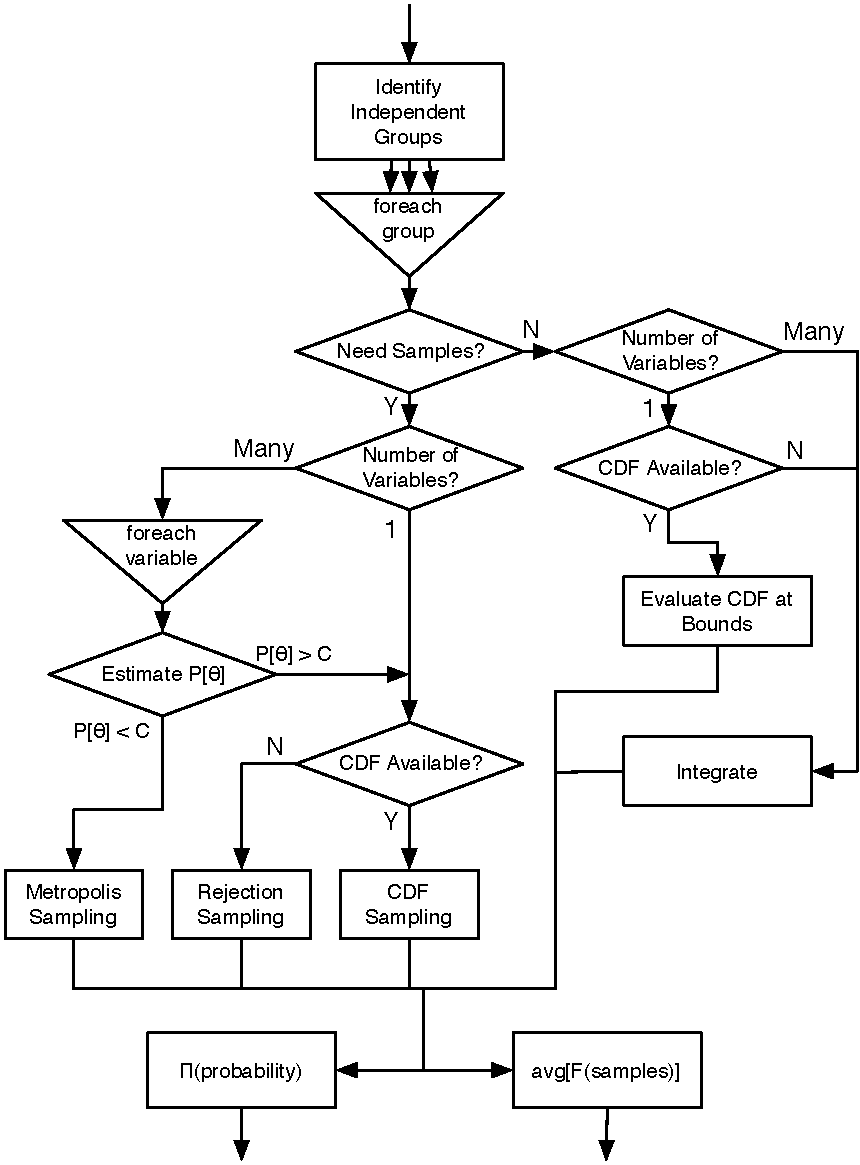
\includegraphics[width=3in]{graphics/roadmap.pdf}
%%\begin{enumerate}
%%\item 
%%\end{enumerate}
%\caption{\textbf{The PIP Single-Row sampling process}}
%\vspace*{-0.2in}
%\label{fig:roadmap}
%\end{center}
%\vspace*{-0.15in}
%\end{figure}


\subsection{Aggregate Sampling Operators}
Aggregate operators (eg. sum, avg, stddev) applied to c-tables introduce a new form of complexity into the sampling process: the result of an aggregate operator applied to a c-table is difficult to represent and sample from.  Even if the values being aggregated is a constant, each row's context must be evaluated independently.  The result is $2^n$ possible outputs, each with a linear number of conditions in the number of rows.  If the values being aggregated are variable expressions, the result is an identical number of outputs, each containing data linear in the size of the table.  

This added complexity, coupled with the frequency with which they appear at the root of a query plan, makes them an ideal point at which to perform sampling.  As aggregates compute expectations over entire tables, the probability of a given row's presence in the table can be included are included in the aggregate's expectation.  This behavior is termed \textit{per-table sampling semantics}.

We begin with the simplest form of aggregate expectation, that of an aggregate that obeys linearity of expectation ($E[f(\vec{y})] = f(\vec{E[y]})$), such as sum().  Such aggregates are straightforward to implement: per-row expectations of $f(\vec y)\chi(\vec y)$ are computed, and aggregated (e.g., summed up).  Of note however, is the effect that the operator has on the variance of the result.  In the case of sum(), each expectation can be viewed as a Normally distributed random variable with a shared, predetermined variance.  By the law of large numbers, the sum of a set of $N$ random variables with equal standard deviation $\sigma$ has a variance of $\frac{\sigma}{\sqrt{N}}$.  In other words, when computing the expected sum of $N$ variables, we can reduce the number of samples taken for each individual element by a factor of $\frac{1}{\sqrt{N}}$.

If the operator does not obey linearity of expectation (e.g., the max aggregate), the aggregate implementation is made more difficult.  Any aggregate may still be implemented naively by evaluating it in parallel on a set of sample worlds instantiated prior to evaluation.  This is a worst-case approach to the problem; it may be necessary to perform a second pass over the results if an insufficient number of sample worlds are generated.  However, more efficient special case aggregates, specifically designed to compute expectations are possible.


For example, consider the max() aggregate.  If the target expression is a constant, this aggregate can be implemented extremely efficiently.  Given a table sorted by the target expression in descending order, PIP estimates the probability that the first element in the table (the highest value) is present.  The aggregate expectation is initialized as the product of this probability and the first element.  The second term is maximal only if the first term is not present; when computing the probability of the second term, we must compute the probability of all the second term's constraint atoms being fulfilled while at least one of the first atom's terms is not fulfilled.  Though the complexity of this process is exponential in the number of rows, the probability of each successive row being maximal drops exponentially.  

\begin{example}\em
To illustrate this, consider the table (annotated with probabilities)
\[
\begin{tabular}{c|c|c|c}
R & $A$ & $\phi$ & $P[\phi]$\\
\hline
& 5 & $X \ge 7$ & 0.7 \\
& 4 & $Y \ge 7$ & 0.8  \\
& 1 & $Z \ge 7$ & 0.3  \\
& 0 & $Q \ge 7$ & 0.6  \\
\end{tabular}
\]
Based on the probabilities listed above,
$$E[\max(A)] = 5 \cdot 0.7 + 4 \cdot 0.8 + 1 \cdot 0.3 + 0 \cdot 0.6$$
However, if the desired precision is $0.1$, we can stop scanning after the second record since the maximum any later record can change the result is $1-(1-0.7)*(1-0.8) = 0.056$.

\end{example}



%Thus, it only requires a number of steps logarithmic in the precision required.




